\documentclass{sigchi}
% Use this command to override the default ACM copyright statement
% (e.g. for preprints).  Consult the conference website for the
% camera-ready copyright statement.

%% HOW TO OVERRIDE THE DEFAULT COPYRIGHT STRIP --
%% Please note you need to make sure the copy for your specific
%% license is used here!
% \toappear{
% Permission to make digital or hard copies of all or part of this work
% for personal or classroom use is granted without fee provided that
% copies are not made or distributed for profit or commercial advantage
% and that copies bear this notice and the full citation on the first
% page. Copyrights for components of this work owned by others than ACM
% must be honored. Abstracting with credit is permitted. To copy
% otherwise, or republish, to post on servers or to redistribute to
% lists, requires prior specific permission and/or a fee. Request
% permissions from \href{mailto:Permissions@acm.org}{Permissions@acm.org}. \\
% \emph{CHI '16},  May 07--12, 2016, San Jose, CA, USA \\
% ACM xxx-x-xxxx-xxxx-x/xx/xx\ldots \$15.00 \\
% DOI: \url{http://dx.doi.org/xx.xxxx/xxxxxxx.xxxxxxx}
% }
\toappear{}

% Arabic page numbers for submission.  Remove this line to eliminate
% page numbers for the camera ready copy
% \pagenumbering{arabic}

% Load basic packages
\usepackage{balance}       % to better equalize the last page
\usepackage{graphics}      % for EPS, load graphicx instead 
\usepackage[T1]{fontenc}   % for umlauts and other diaeresis
\usepackage{txfonts}
\usepackage{mathptmx}
\usepackage[pdflang={en-US},pdftex]{hyperref}
\usepackage{color}
\usepackage{booktabs}
\usepackage{textcomp}

\usepackage[
    backend=biber,
    style=draft
]{biblatex}

\addbibresource{paper.bib}


% Some optional stuff you might like/need.
\usepackage{microtype}        % Improved Tracking and Kerning
% \usepackage[all]{hypcap}    % Fixes bug in hyperref caption linking
\usepackage{ccicons}          % Cite your images correctly!
% \usepackage[utf8]{inputenc} % for a UTF8 editor only

% If you want to use todo notes, marginpars etc. during creation of
% your draft document, you have to enable the "chi_draft" option for
% the document class. To do this, change the very first line to:
% "\documentclass[chi_draft]{sigchi}". You can then place todo notes
% by using the "\todo{...}"  command. Make sure to disable the draft
% option again before submitting your final document.
\usepackage{todonotes}

% Paper metadata (use plain text, for PDF inclusion and later
% re-using, if desired).  Use \emtpyauthor when submitting for review
% so you remain anonymous.
\def\plaintitle{Why did they win?\\Visualizing NBA teams across multiple seasons}
\def\plainauthor[#1]{#1}
\def\plainauthors[#1]#2#3{#1, #2, #3}
\def\emptyauthor{}
\def\plainkeywords{Information Visualization; CHI; NBA}
\def\plaingeneralterms{}

% llt: Define a global style for URLs, rather that the default one
\makeatletter
\def\url@leostyle{%
  \@ifundefined{selectfont}{
    \def\UrlFont{\sf}
  }{
    \def\UrlFont{\small\bf\ttfamily}
  }}
\makeatother
\urlstyle{leo}

% To make various LaTeX processors do the right thing with page size.
\def\pprw{8.5in}
\def\pprh{11in}
\special{papersize=\pprw,\pprh}
\setlength{\paperwidth}{\pprw}
\setlength{\paperheight}{\pprh}
\setlength{\pdfpagewidth}{\pprw}
\setlength{\pdfpageheight}{\pprh}

% Make sure hyperref comes last of your loaded packages, to give it a
% fighting chance of not being over-written, since its job is to
% redefine many LaTeX commands.
\definecolor{linkColor}{RGB}{6,125,233}
\hypersetup{%
  pdftitle={\plaintitle},
% Use \plainauthor for final version.
  pdfauthor={\plainauthors[Yannick Boesmans]{Yannick Laevaert}{Yves Langeraert}},
%  pdfauthor={\emptyauthor},
  pdfkeywords={\plainkeywords},
  pdfdisplaydoctitle=true, % For Accessibility
  bookmarksnumbered,
  pdfstartview={FitH},
  colorlinks,
  citecolor=black,
  filecolor=black,
  linkcolor=black,
  urlcolor=linkColor,
  breaklinks=true,
  hypertexnames=false
}

\pagenumbering{arabic}

% create a shortcut to typeset table headings
% \newcommand\tabhead[1]{\small\textbf{#1}}

% End of preamble. Here it comes the document.
\begin{document}

\title{\plaintitle}

\numberofauthors{3}
\author{%
  \alignauthor{\plainauthor[Yannick Boesmans]\\
    \affaddr{KU Leuven}\\
    \email{yannick.boesmans}\\
    \email{@student.kuleuven.be}}\\
  \alignauthor{\plainauthor[Yannick Laevaert]\\
    \affaddr{KU Leuven}\\
    \email{yannick.laevaert}\\
    \email{@student.kuleuven.be}}\\
  \alignauthor{\plainauthor[Yves Langeraert]\\
    \affaddr{KU Leuven}\\
    \email{yves.langeraert}\\
    \email{@student.kuleuven.be}}\\
}

\maketitle

\begin{abstract}
    In this paper we describe an interactive visualization of the NBA competition over the last 30 years. With three different views, we give the opportunity for the user to explore various kinds of data about NBA seasons including standings, team statistics, transfers and player statistics. The d3.js framework was used to develop this visualization.
    %TODO add results
    
    
    

\end{abstract}

%TODO keywords
\category{H.5.m.}{Information Interfaces and Presentation
  (e.g. HCI)}{Miscellaneous} \category{See
  \url{http://acm.org/about/class/1998/} for the full list of ACM
  classifiers. This section is required.}{}{}

\keywords{\plainkeywords}

\section{Introduction}

The National Basketball Association (NBA) is the most famous and perhaps the best professional basketball league in the world. Like in every other sports branch, a lot of data and statistics about players, teams, games and seasons are available, mainly in large tables. Despite these tables contains a lot of information, it is very hard if not impossible, to interpret, compare efficiently and gather insights in it. In our work we try to present this data in a whole different way. Therefore we have focused ourselves on some parts and not the entire available data.

This paper describes the visualization of NBA data made by the ``The Tufters''
team for the course ``Information Visualization''. In section~\ref{sec:goal} we
describe the goal of the visualization and the target audience. In
section~\ref{sec:data} we describe the data used, including its origins,
advantages and limitations. In section~\ref{sec:literature} we give an overview
of related literature and web resources, including related visualizations.  This
includes both visualizations of NBA or other sports data, as well as
visualizations tackling an isue encountered during the development of our
visualization. In section~\ref{sec:visualization} we describe the visualization
itself. We give an overview of the different stages of development of the
visualization, as well as the major design decisions.
Section~\ref{sec:discussion} discusses potential improvements of the final
visualization and lessons learned from the project. We conclude in
section~\ref{sec:conclusion}. Appendix~\ref{sec:terminology} contains
definitions for common basketball terms used in this paper.

\section{Goal and Target Audience}\label{sec:goal} 
The visualization's goal can be best summarized by the following sentence: ``Why
did a certain NBA-team win the Championship?'' The visualization focuses on exposing relations between team
performance and their player roster over several years. It allows users to find
explanations for major improvements and declines in team performance.  The
visualization allows exploration of NBA data by lay persons.  More specifically,
the visualization does not focus on premade explanations for phenomenons
visible in the NBA data. By providing easy and intuitive access to the data, the
visualization allows users to draw their own conclusions. The visualization's
target audience are lay persons. Specifically, fans of NBA are the core of our
target audience. This means the visualization assumes most common basketball
terms are known to the audience and does not provide basic terminology
explanations. 
< We also give basic insights in why a statistic changes (arrow views)
we try to help them explore patters and trigger them for questions
Do we create awareness?
>

\section{Data}\label{sec:data}
The data visualized is a subset of the data available on basketball statistics
site basketball-reference\cite{basketball-reference}. A wide range of data is
available on this site. This includes common basketball performance statistics,
such as field goals, percentage of shots scored, shooting distance, minutes
played per season, number of personal fouls made, salaries and much more. These
statistics are avalable for each player individually for each season. Aggregated
data for entire teams and for entire seasons is also available. Additionally,
individual game statistics are also available, including playoff games.  In our
visualization we only use data from 1984 onwards. This is done because of rule
changes in the NBA which changed the number of teams competing and the
competition's structure. To simplify implementation of our visualization, only
data after the last major rule change was used.  The data we use includes league
standings and playoff rankings for each team, team overall statistics, the
team's roster and individual player statistics for each year, including the
PER~(Player Efficiency Rating)\cite{per}. 

The data was gathered by scraping the basketball-reference site using the
provided download capabilities. Most of the data was downloaded in csv format,
while some tables had to be manually scraped. This process was automated using
Python scripts. The data was then combined in a preprocessing step. In this
step, each team's playoff rankings were calculated based on the matches played
during the playoffs, and the rest of the data was combined into json format. The
final preprocessing step combined all data into one json file.

<Tell something more about the data in terms of tall/wide data
Mention that it's a time series
Tell something more about pre-processing steps (why?, did we change it over time?)
rfr to picture in 1st ppt sl 60>

\begin{figure}
\centering
  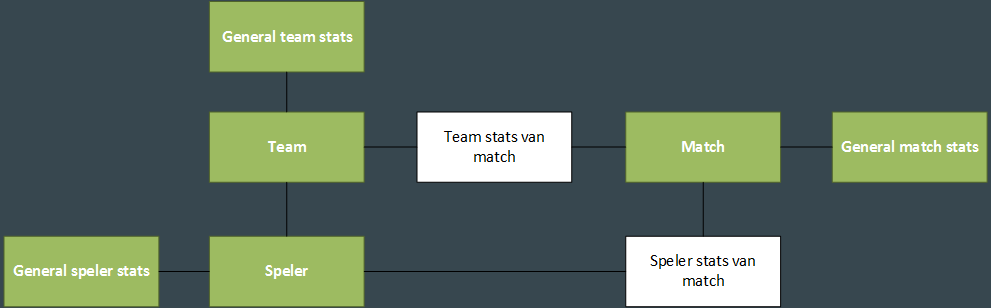
\includegraphics[width=0.9\columnwidth]{figures/data}
  \caption{An overview of the data.}~\label{fig:data}
\end{figure}

\section{Related Work}\label{sec:literature}

On the IEEE Visualization Conference in 2013, the first workshop on sports data visualization was held \cite{ieeevis}. There is shown that the area of sport produces large amounts of data, which can be used for building visualizations and making analyses of the data. In the past visualizations of sports existed already, but there were not a lot of visualizations, and they were simple in the sense that they just represented the data without trying to give insights or to approach the data on a different way. There are some, but limited, sports-specific visualizations, like the basketball shot chart. This is a visualization frequentely seen when looking for visualizations about the NBA. Some shot chart vizualisations try to be different than others, but the general design and idea stays roughly the same. 
% 2 goeie papers die hierin verwerkt kunnen worden
%http://www.sloansportsconference.com/wp-content/uploads/2012/02/Goldsberry_Sloan_Submission.pdf
%http://vis.berkeley.edu/courses/cs294-10-sp10/wiki/images/archive/a/a2/20100511091342!Stephen_Chu_-_Information_Visualization_in_the_NBA_-_The_Shot_Chart_16.pdf

With our visualization we try to make it easier to interpret a collection of data about the NBA, and try to let users find patterns and insights in the data. A same kind of incentive was the start for \cite{cox2006sportsvis} who created a visualization to help people discover meaning in statistics generated during sporting events in the case of baseball.



%Related work/References

%Shot charts
%http://peterbeshai.com/buckets/app
%http://vorped.com/1-nba/2015-2016/player/6667/emmanuel-mudiay/
%https://github.com/amatlin/NBAvis
%https://thedatagame.com.au/2015/09/27/how-to-create-nba-shot-charts-in-r/
%http://savvastjortjoglou.com/nba-shot-sharts.html?utm_source=Python+Weekly+Newsletter&utm_campaign=5185ff0538-Python_Weekly_Issue_202_July_30_2015&utm_medium=email&utm_term=0_9e26887fc5-5185ff0538-312727397
%http://toddwschneider.com/posts/ballr-interactive-nba-shot-charts-with-r-and-shiny/

%Standings
%https://source.opennews.org/en-US/articles/nyts-512-paths-white-house/
%http://projects.fivethirtyeight.com/complete-history-of-the-nba/#warriors
%http://www.theguardian.com/news/datablog/interactive/2013/jun/03/premier-league-season-visualised
%http://gizmodo.com/5927503/all-the-major-sport-competitions-since-1903-condensed-in-beautiful-circular-graphics
%http://www.nbaplayoffsbracket.com/2016/index.php
%http://nyloncalculus.com/2015/08/07/as-nba-empires-rise-and-fall/
%http://inf.ufrgs.br/~lsguedes/skooth/Publications_&_Works_files/nbavis_final.pdf
%http://research.microsoft.com/pubs/64282/tvcg2007-adaptivitree.pdf
%http://www.student.kuleuven.be/~s0217391/mume/deliverables/paper.pdf

%Other
%https://graphics.stanford.edu/wikis/cs448b-10-fall/FP-RuthEric-HeddlestonKate?action=AttachFile&do=get&target=448bPaper.pdf
%http://www.scribblelive.com/blog/2014/03/20/the-power-of-sports-data-visualizing-passes-between-nba-players-offers-new-game-insights/
%http://lemonchiu.github.io/NBA-Visualization/


\section{Visualization}\label{sec:visualization}
The visualization consists of three parts:
\begin{itemize}
    \item The play-off view: a compact view on the play-offs per season
    \item The statistics (zoom) view: a more detailed view on a statistic of a selected team
    \item The team view: a detailed view on how good or bad a team scores on a specific field position
\end{itemize}

\begin{figure}
\centering
  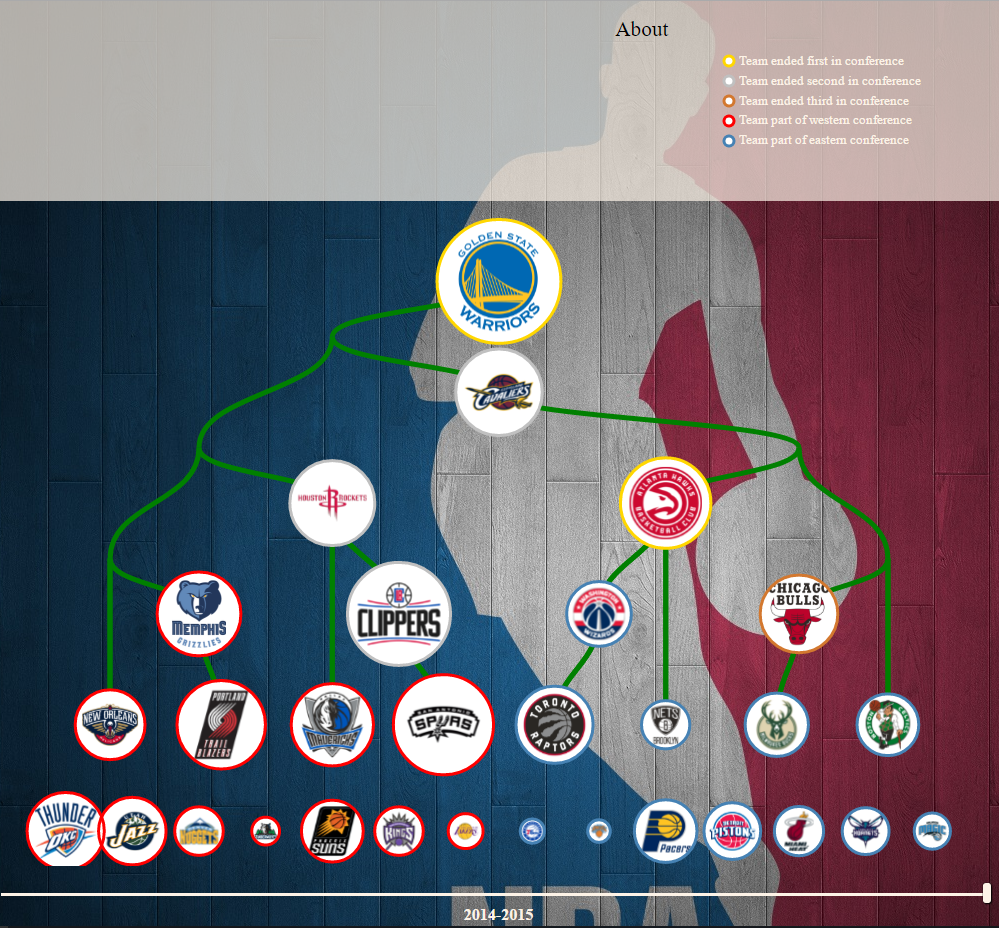
\includegraphics[width=0.9\columnwidth]{figures/playoffviewwithcontext}
  \caption{The play-off view without a team selected.}~\label{fig:playoffviewnoteam}
\end{figure}

\begin{figure}
\centering
  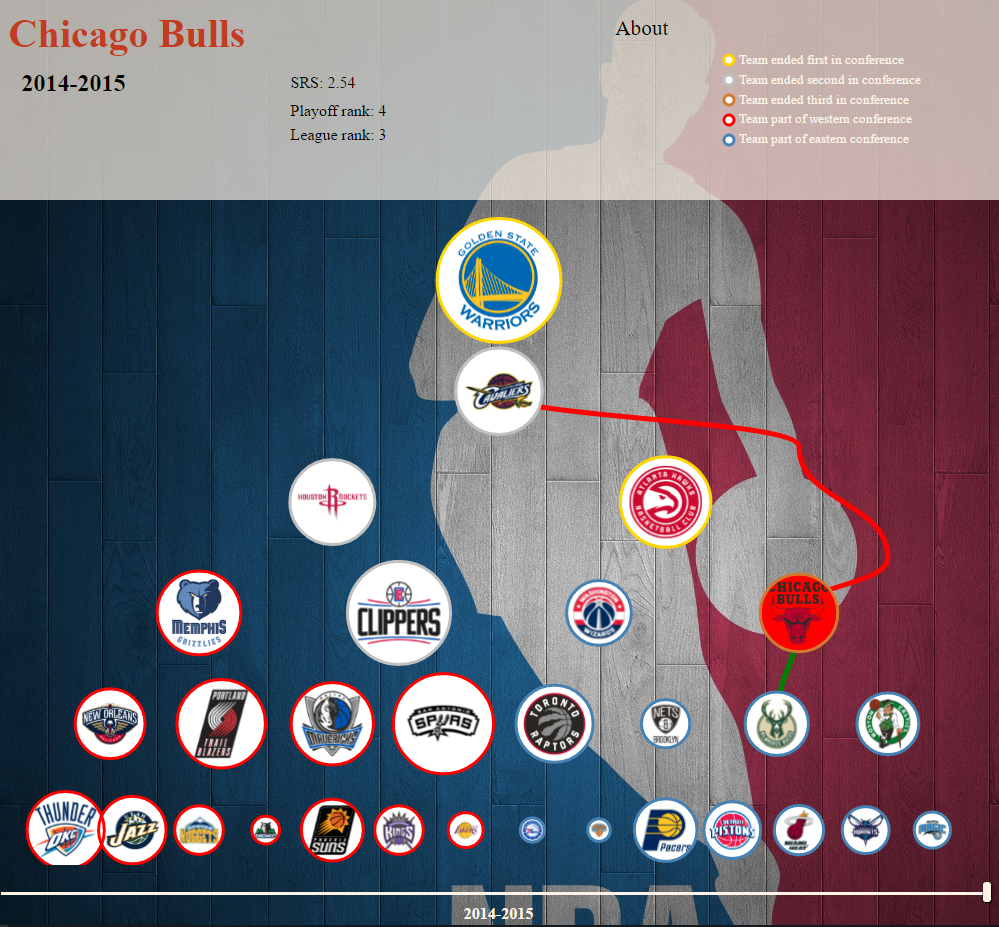
\includegraphics[width=0.9\columnwidth]{figures/playoffviewteamselected}
  \caption{The play-off view with a team selected.}~\label{fig:playoffviewteam}
\end{figure}

\begin{figure}
\centering
  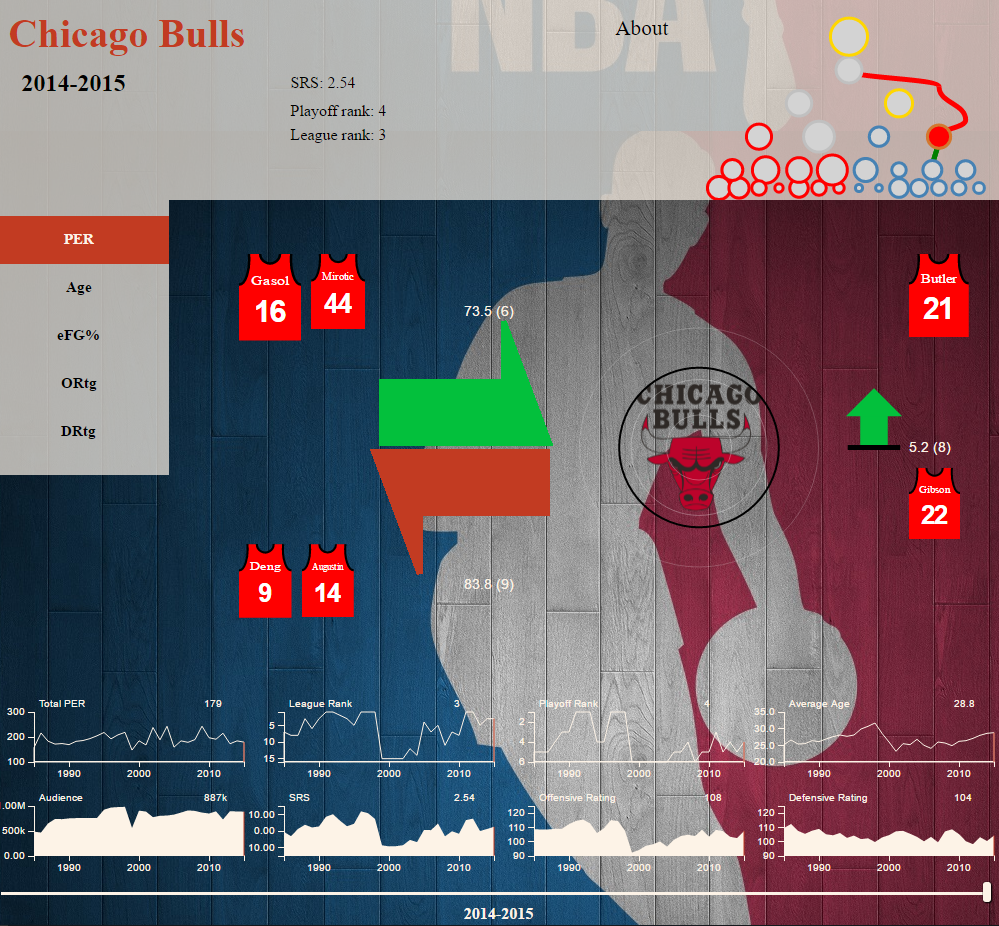
\includegraphics[width=0.9\columnwidth]{figures/statisticsview}
  \caption{The statistics view.}~\label{fig:statisticsview}
\end{figure}

\begin{figure}
\centering
  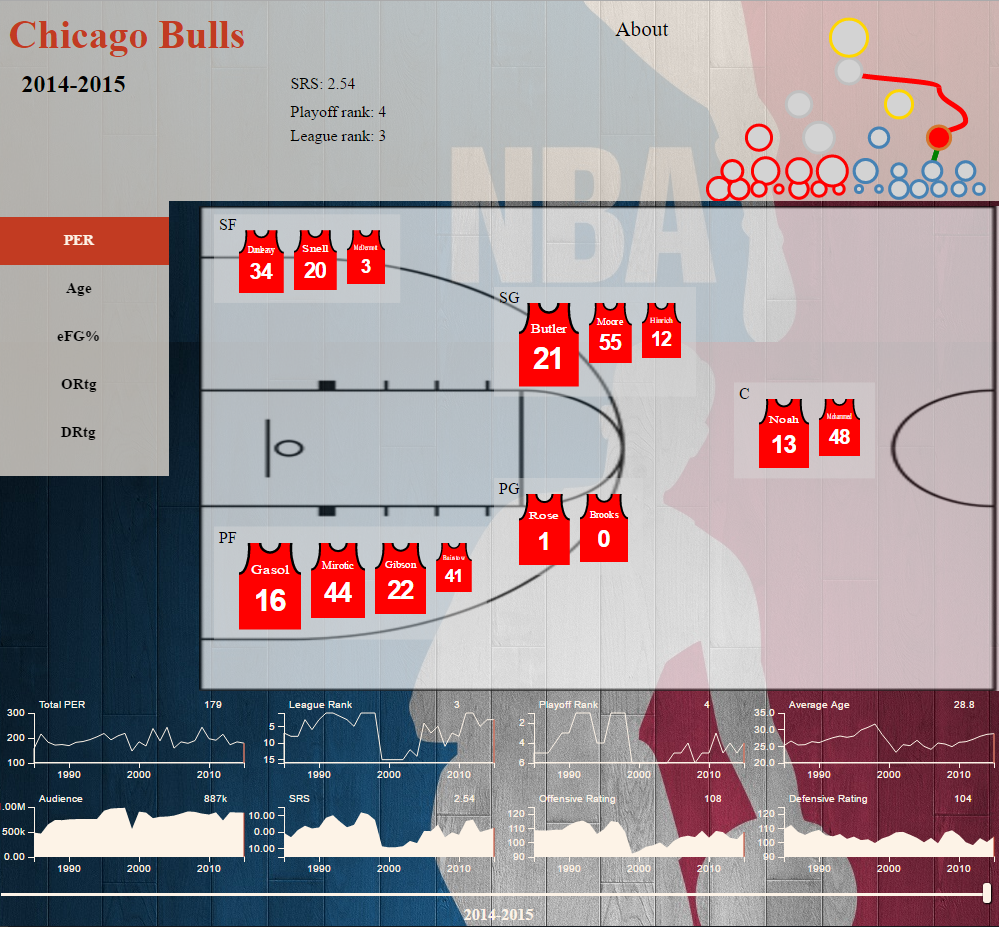
\includegraphics[width=0.9\columnwidth]{figures/teamview}
  \caption{The team view.}~\label{fig:teamview}
\end{figure}

<Explain that this complies with the infovis seeking mantra: Overview, zoom&filter, details on demand
play-off view = overview
statistics view= details on demand
Talk about th organization of the 3 views + the choice for a tiled approach
- Each page is a 'tile' that we force with fixed scrolling
- Use of the keyboard is possible (space bar to scroll + arrows, arrows for timeline)
- This papers are usefulle to refer to
http://courses.ischool.berkeley.edu/i247/f05/readings/Baldonado_MultipleViews_AVI00.pdf
http://www.interactiondesign.us/courses/2011_AD690/PDFs/Shneiderman_1996.pdf
http://www2.parc.com/istl/groups/uir/publications/items/UIR-1986-02-Mackinlay-TOG-Automating.pdf
>

All three are discussed in more detail below. The three views are available to
the user on a single webpage. The user start on the play-off view and is able to
navigate to the statistics and team views by scrolling down or clicking on
teams. A different season can be selected with the left and right arrows or by clicking on the timeline. The timeline is a fixed part of the visualization, hence visible in the three different views.
%The webpage is built in such a way that it gives a hint to the user at the bottom
%or the top of a page when another view is available. By showing a different 
%background color and an arrow, we invite the visitor to explore other views. The 
%user is also at liberty to scroll through these views. However, a fixed scroll is
%implemeted so users will only end in complete views when moving around. Note that 
%the user also will be guided through all 3 views when performing actions described 
%in the section below.

\subsection{The play-off view}
This view informs the user of the roster and end positions in the NBA play-offs for a selected season, in general or for a selected team. The view consists of two parts: 
\begin{itemize}
    \item Context section: the top part informs the user about the selected team and shows a legend of the play-off view.
    \item Bubble section: this section represents the play-offs of the selected season
\end{itemize}
The play-off view is shown in Figure~\ref{fig:playoffviewwithcontext}.

\subsubsection{Context section}
The context section contains a legend that explains the stroke colors used in the bubble section. The stroke is gold, silver or bronze if the team ended respectively first, second or third in the regular competition. Teams that didn't end in a podium place during the regular competition have a red or blue stroke color indicating the team's region, respectively the western or eastern conference. The context section also contains a link to another page (``About'') where the user can get an explanation of the visualization with its different views, can get some background information about the NBA and the terminolgy used, and can check the source of our used data. If the user hovers over or selects a team in the bubble section, the context section shows more information about that team, as shown in Figure~\ref{fig:playoffviewteamselected}. This includes the Simple Rating System score (SRS), the end position in the play-offs and the end position in the regular competition.

\subsubsection{Bubble section}
This section presents the roster and end positions of the play-offs for a selected season. Every team is respresented by a circle with the logo of the team inside it. Our initial desing filled the circle with the logo of the team and colored the circle red or blue depending on the region where the team competed. The shade of colour was darker if their final ranking was higher in their region. According to the Ranking of Perceptual Tasks~\cite{perceptualranking} this is a good property for ordered values like the regular competition ranking. But the combination of the logo's of the teams with the colors made it to heavy and less easy to compare the end ranking of different teams. As an alternative we tried the same view without the logo's, but this is inconvenient because you don't know which team is represented by which circle. Therefore we've chosen to only use the logo's of the teams as we thought this is more user friendly and the extra information of the ranking doesn't outweight. The size of the circle represents the SRS score using an own interpretation of perceptual scaling because the (Flannery) Appearance Compensation is not usable with a domain of both negative and positive values. An exponential function with exponent 1.5 was used. This way the proportion between the area of a bigger and the area of a smaller circle will be greater than the proportion of values the areas represent. The stroke of the circle illustrates the team's region or medal won during the regional competition as explained in the context section. The curved lines between teams represent that those teams have encountered each other in the playoffs. Each row represents an end position in the play-offs. The higher a team is, the further it has come. From the top to the bottom the rows represent the winner of the final (place 1), loser of the final (place 2), losers of the semi-finals (place 3), losers of the quarter-finals (place 4), losers of the 1/8-finales (place 5). The last row represents the teams that did not make it to the play-offs (place 6).  A connection is always made between a team that is in a higher row and a team that is in a lower row. The highest team of the two teams has won the confrontation, and therefor went at least one round further in the play-offs. The two up most teams are the winners of the play-offs in their own conference and played the final. 
A more popular visualization of a play-off is the team double elimination bracket.
Although this is a more common representation , and there are some nice desings like in this NBA 2012 play-offs visualisation~\cite{tournamentladder} where a sunburst visualisation is used, we wanted to create a more compact version by eliminating the recurring representation of a team. We considered enclosed circles, as used in this visualisation of the wimbledon tournament roster~\cite{enclosedcircles}.
Although the enclosed circles is a compact representation as well, we have continued 
with our own design as we believe this view is more original and innovative. Furthermore we are convinced that our view gives a good illustration of the end positions. It's generally assumed that the team that is on top of the ``ladder'' is the winning team. We didn't encouter a similar view when searching for alternatives to visualize a play-off or championship. A new visualization has the advantage that it will trigger users as well.

<Talk about the importance of estethics seen in the lesson>
Our initial play-off view was too heavy. It connected teams that played against
each other directly. When searching for alternatives to reflect on our choice we
discovered a similar visualization in a totally different context. 
<https://source.opennews.org/en-US/articles/nyts-512-paths-white-house/>
<comparison of original play-off view with white house paths>
This visualization gives a cleaner view of the competitors for a specific team
compared to our original sketch. Hence we decided to adapt our visualization. We
added an intermediate step between two teams to clearer indicate how teams competed
to become NBA champion.
Next to the static view, the user can interact with the visualization. When he 
hoovers over a circle of a team, only the games played by that team are shown by highliting the 
competitors (their circles) and the curved lines that connect them. This view gets 
fixated when the users clicks on a team.
He/she then automatically gets forwarded to the statistics view where the play-off 
view is still represented in the right upper corner to make sure the user keeps
an overview. The statistics view will be explained in more detail in the next section.


< Hierarchy = sorting = facilitate trends of winners
position have a meaning in the play-off view
when selecting circle => zoom/more detail
Bubble principle of 
- Symmetry (whole = play-off)
- conectedness arc = games played
Pre attentive characteristics
- size of circles
- hue to highligt selections or indicate increase decline arrows next view

We considered a map view to just show the teams and there regular competition ranking. But this was a view that has no additional value in comparison with the play-off view except for the geographical position, which has no importance for our visualisation. Furthermore we've found a visualisation of the NBA with a map view~\cite{mapviewvisualization} similar to our idea, so we decided to not implement this map view. 

This visualization helped us discover data quality issues => cut off year 1984
>


\subsection{The statistics view}
The statistics view gives a user a clear overview of how a statistic has been influenced in the selected season compared to the season before. The statistics view is showed in Figure~\ref{fig:statisticsview}. The view consists of 3 coordinated parts:
\begin{itemize}
    \item Context section: the top part informs the user of the context of the selected team
    \item Arrow section: this section illustrates why a statistic changed compared to the previous season
    \item Small multiples section: small multiples of team statistics and how they evolve over time
\end{itemize}

\subsubsection{Context section}
The context section informs the user at all times of the current selection of a team  
that have been made in the play-off view. The statistics view will always be based on a specific team and season that have been selected or that are initated. This should be clear based on the textual information in the top left. Next to that, in the top right a small play-off view is shown. It indicates the team selected and how well it performed in  the play-offs during that season, as explained in the play-off view section. When changing teams and/or season, this view gets updated as well as the textual information. <Explain that the context supports the short term memory of human beings rfr. Monkey Illusion>


\subsubsection{Arrow section of selected statistic}
This section illustrates a change for a chosen statistic for the selected team compared with the season before. This should give a visitor more insight into why a statistic changed over time. The selected team is represented by a circle in the same way as explained in the play-off view. The change for a statistic is represented by three arrows:
\begin{itemize}
    \item Arrow on the left pointing towards the circle: indicating the influence of players who joined the team (team member current season, not previous season)
    \item Arrow on the right of the circle: indicating how the team inherent changed (team member this season and previous season)
    \item Arrow on the left pointing away from the circle: indicating the influence of players who left the team (team member previous season, not current season)
\end{itemize}
<figure of the statistics view>
The shirts next to the arrows are the shirts of players that had the biggest 
contribution to that arrow. Note that these shirts don't change in size. The box on 
the right enables the user to change between 
statistics. Next to that it informs the user of which statistic has been chosen. When 
the user hits the circle in the middle representing the teams, he is guided 
to the team view. This view will be explained in more detail in the next section.
<filtering: 
- time & team
- based on exploration (small multiples)
- dynamically: changes impact multiple parts>

\subsubsection{Small multiples of different statistics}
Below the arrow section small multiples are shown of multiple statistics over time. 
The line charts enables a user to identify peaks or drops that possibly influenced the 
outcome of a team is this season, following seasons or previous seasons. A user interacts with the visualization by shifting the bar indicating the current year displayed. By doing this the view gets updated and the user can see the impact on the team in the context section and why the statistic changes in the arrow section. An alternative to scroll through time is to use the timeline at the bottom of the page.
<this vis helps us comparre statistics over time and relations between them
eg. srs score & play-off ranking>

\subsection{The team view}
This view as well as the statistics view should give the user the ability to search
for explanations why a team is is performing better or worse over seasons. On the 
other hand, a user can see what impact a change in team characteristics has on its
overall performance.
This view shows each player of the team on its field positions. Shirts aligned next to 
each other will thus share the same position. The size of a shirt would illustrate a players performance on this spot. The PER score is initiated. This view should give
a user insight on how strong or weak a particular team is for a specific field position.
A user can then scroll through time, see how field positions evolve and what the influence
is over time.
Initially we designed this view more elaborate. When the user would click on a shirt,
specific player information would be shown. Next to some general text information, 
we would have visualised a number of player statistics as small multiples. A bell curve
should have informed how a player scores compared to his team, other players in the 
league on this position or all other players in the league. We considered other charts for
the small multiples as well. A box plot or bullet was less clear for us to indicate where
a player stands compared to the group he was compared with. Alternatives for the small 
multiples were evaluated as well. One good alternative was the shooting signature.\cite{peterbeshai}
However, creating such a visualization is again a project on itself and due to time 
constraints we left it aside. Other possibilities such as a heatmap or spider web didn't
fulfill our need to give the visitor a clear overview of how a player performed compared
to its peergroup.
<Sketch of the small multiples>

\subsection{Improving the result}
Talk about how we improved the data-ink ration in the end..

\section{Possible improvements}
As with most projects, the result is never 'finished', meaning that there are always improvements
possible but due to timing or resource constraints the haven't all been implemented. In what 
follows, we suggest a number of features that might improve the visualization:
\begin{itemize}
    \item Smooth transitions between states could improve the user experience. For example when changing
    year, a transformation of the arrow in the statistics view would help the user see a difference between years.
    At the moment the arrows change at the blink of an eye, making it difficult for us humans with a short term memory
    to make the comparison.
    \item To further support our short term memory we could also 'save' the previous state. Eg. in the field view we could
    visualize ghost shirts to indicate which players left the team or position and highlight players that joined the team. 
    This would help the user see how the team changes over time.
    \item At the moment no attention has been payed to the process & provenance of the exploration. A user thus needs to 
    memorize his action to be able to share or reproduce his actions. This could be improved by adding URL parameters. This
    way a user at least can share or save a state of an analysis. One step further is to provide a play-feature. The visitor could 
    them share his exploration and replay it. A simple implemention would ask the visitor for a start date and an end date and
    would then 'play' the changes of a particular team and characteristic over time.
    \item We could support users further in exploring for patterns by focussing more on comparisons. We could integrate a view 
    where a visitor is able to compare two teams in the same year, or in two different years.
\end{itemize}

\subsection{Technology}
To create the visualization, the d3 javascript framework~\cite{d3.js} was used in combination with html5~\cite{html5} and jquery~\cite{jquery}.  Note that D3 is based on HTML, CSS, Javascript and SVG.
Next to that,the use of D3 was a requirement for the project. This allows easy
access to the visualization as most modern browsers are capable of handling
these webstandards. 
The choice not to use the d3 framework for the entire visualization was made to
ease the layout configuration of the visualization. Instead, html was used to do
the global layout of the visualization. We opted to structure the site with multiple
divs as containers. To each container we allocate a svg with a specific visualization.
Eg. The statistic view is build out of x divs filled with different svg's created
with the d3 framework.
<sketch of how the page is structured>
When working with d3.js we encountered some obstacles:
- A synchrounous call need to be combined with synchronous calls. More specific, when a visitor uses the timeline to scroll through time, the whiping of previous visualizations was not synced with the creation of the visualisation. This resulted in whiping sections when a visualization was not created yet. Hence the view resulted in multiple figures overlapping.


\section{Lessons learned}\label{sec:discussion}
We've learned a couple of lessons during the creation of this visualization:
\begin{itemize}
    \item Find a story to tell with your visualization
    \item Each separate component should be a sufficient informative visualization on itself
    \item Creating a custom visualization costs time and opportunities
\end{itemize}
In what follows we will discuss our experience in more detail.

\subsection{Story telling}
At the beginning of this project we were able to design the 3 separate views 
quite quickly. Our main problem was to integrate these views as a whole. When we created drafts of two views being the play-off view and the statitics view, we suddenly noted patterns. The Golden State Warriors became NBA champion a couple of years after a great uplift in SRS score. This due to a increase inside the team and because of new players joining the team in 2009. In 
the years following, the team kept on attracting talented players and increased the inherent team score (with ups and downs) to become NBA champion in 2015. With the team view, one can even notice that the team gets stronger in center team positions during this period. The visualization however is missing at the moment if this reinforcement of the field positions
is due to the attraction of talented people or by utilizing available talent within the team. Rfr to possible improvements. Being able to visualize this story, enabled us to support visistors in searching their own stories. They are able to explore the data for patters. On top of that, we provide the insight on how the changes were impacted by changes in teamplayers.

\subsection{Each component should be informative}
In order to have a good visualization as a whole, each component should be a clear and 
informative visualization on itself. This is a lesson learned from our work, but also when
evaluating the work of peers. We started noticing that most components in a visualization 
lack references and hence are not informative enough. Eg. each small multiple of a statisctic
in the statistics view on itself gives sufficient information to stand on itselfs. The bar in
the small multiple indicates the score in the selected season and enables the user to evaluate
that score over time. Have there been better scores, or worse scores. Is this score part of 
an upward movement during years? 
For this reason we can argue that the circle representing the teams SRS score in the statisctics
view is not the best choice. We could have chosen a bar chart with an indication of the best and
worst score for that specific team over time or for the best and worst team in that season.

\subsection{Custom visualizations}
Before exploring what is out there in the d3.js world, we made our own sketches. This is how we came up with the 3 custom views that makes our visualization. When comparing our design with alternatives we could not find something that satisfied our needs. Nonetheless, they gave us inspiration to finetune our designs. Although we are satisfied with our result and we are convinced it was the right choice to reach our goal, it had some draw backs.
We noted that other teams had more freedom in exploring multiple different visualizations which enabled them to evaluate different options with trial and error. We could have prepared our data in a format that was more compatible with out of the box examples, but this would have had too much of an impact on our result.
<Talk about redesign>
Next to that, although we've tried to write our code as general as possible, we're not convinced this could be shared in such a way that other people building a visualization could easily re-use our work to visualize other sports.

\section{Conclusion}\label{sec:conclusion}


% Balancing columns in a ref list is a bit of a pain because you
% either use a hack like flushend or balance, or manually insert
% a column break.  http://www.tex.ac.uk/cgi-bin/texfaq2html?label=balance
% multicols doesn't work because we're already in two-column mode,
% and flushend isn't awesome, so I choose balance.  See this
% for more info: http://cs.brown.edu/system/software/latex/doc/balance.pdf
%
% Note that in a perfect world balance wants to be in the first
% column of the last page.
%
% If balance doesn't work for you, you can remove that and
% hard-code a column break into the bbl file right before you
% submit:
%
% http://stackoverflow.com/questions/2149854/how-to-manually-equalize-columns-
% in-an-ieee-paper-if-using-bibtex
%
% Or, just remove \balance and give up on balancing the last page.
%
\balance{}

% REFERENCES FORMAT
% References must be the same font size as other body text.
%\bibliographystyle{SIGCHI-Reference-Format}
\printbibliography
%TODO References should be in alphabetical order and represented by numbers in the text.

\appendix
\section{Terminology}\label{sec:terminology}

\paragraph{PER} Player Efficiency Rating - An all-in-one basketball rating,
boiling down all of a player's contributions into one number\cite{per}.

\end{document}

%%% Local Variables:
%%% mode: latex
%%% TeX-master: t
%%% End:
